\documentclass[sigconf,nonacm]{acmart}

\usepackage{graphicx}
\usepackage{booktabs}
\usepackage{amsmath}
\usepackage{multirow}

\begin{document}

\title{Paraphraser Fingerprinting: Can We Identify the Rewriter from the Text Alone?}

\author{Boyuan Zhang | Yange Wang | Yang-ching Liao}
\affiliation{%
  \institution{Northeastern University}
  \city{Seattle}
  \state{WA}
  \country{USA}
}


\maketitle

% ============================================================
\section{Problem Description}
% ============================================================


Our research question is:
\begin{quote}
\textbf{RQ: Paraphraser Fingerprints.} Do different paraphrasing models leave distinct, detectable traces in their outputs? Can we identify the paraphraser from the text alone?
\end{quote}

% ============================================================
\section{Dataset}
% ============================================================

Each experimental run produces 20 trials.
Only the initial trial uses a human-crafted source text containing deliberate linguistic traps (non-standard grammar, intentional repetition, temporal disorder, counting exercises).
All subsequent trials use source texts generated by the Auditor LLM using Automatic Prompt Engineering (APE)-style iterative refinement based on past Detective feedback.

% ============================================================
\section{Experimentation and Results}
% ============================================================

\subsection{Experimental Setup}

% experiment_setup





\subsection{Aggregate Accuracy}

\begin{figure}[t]
    \centering
    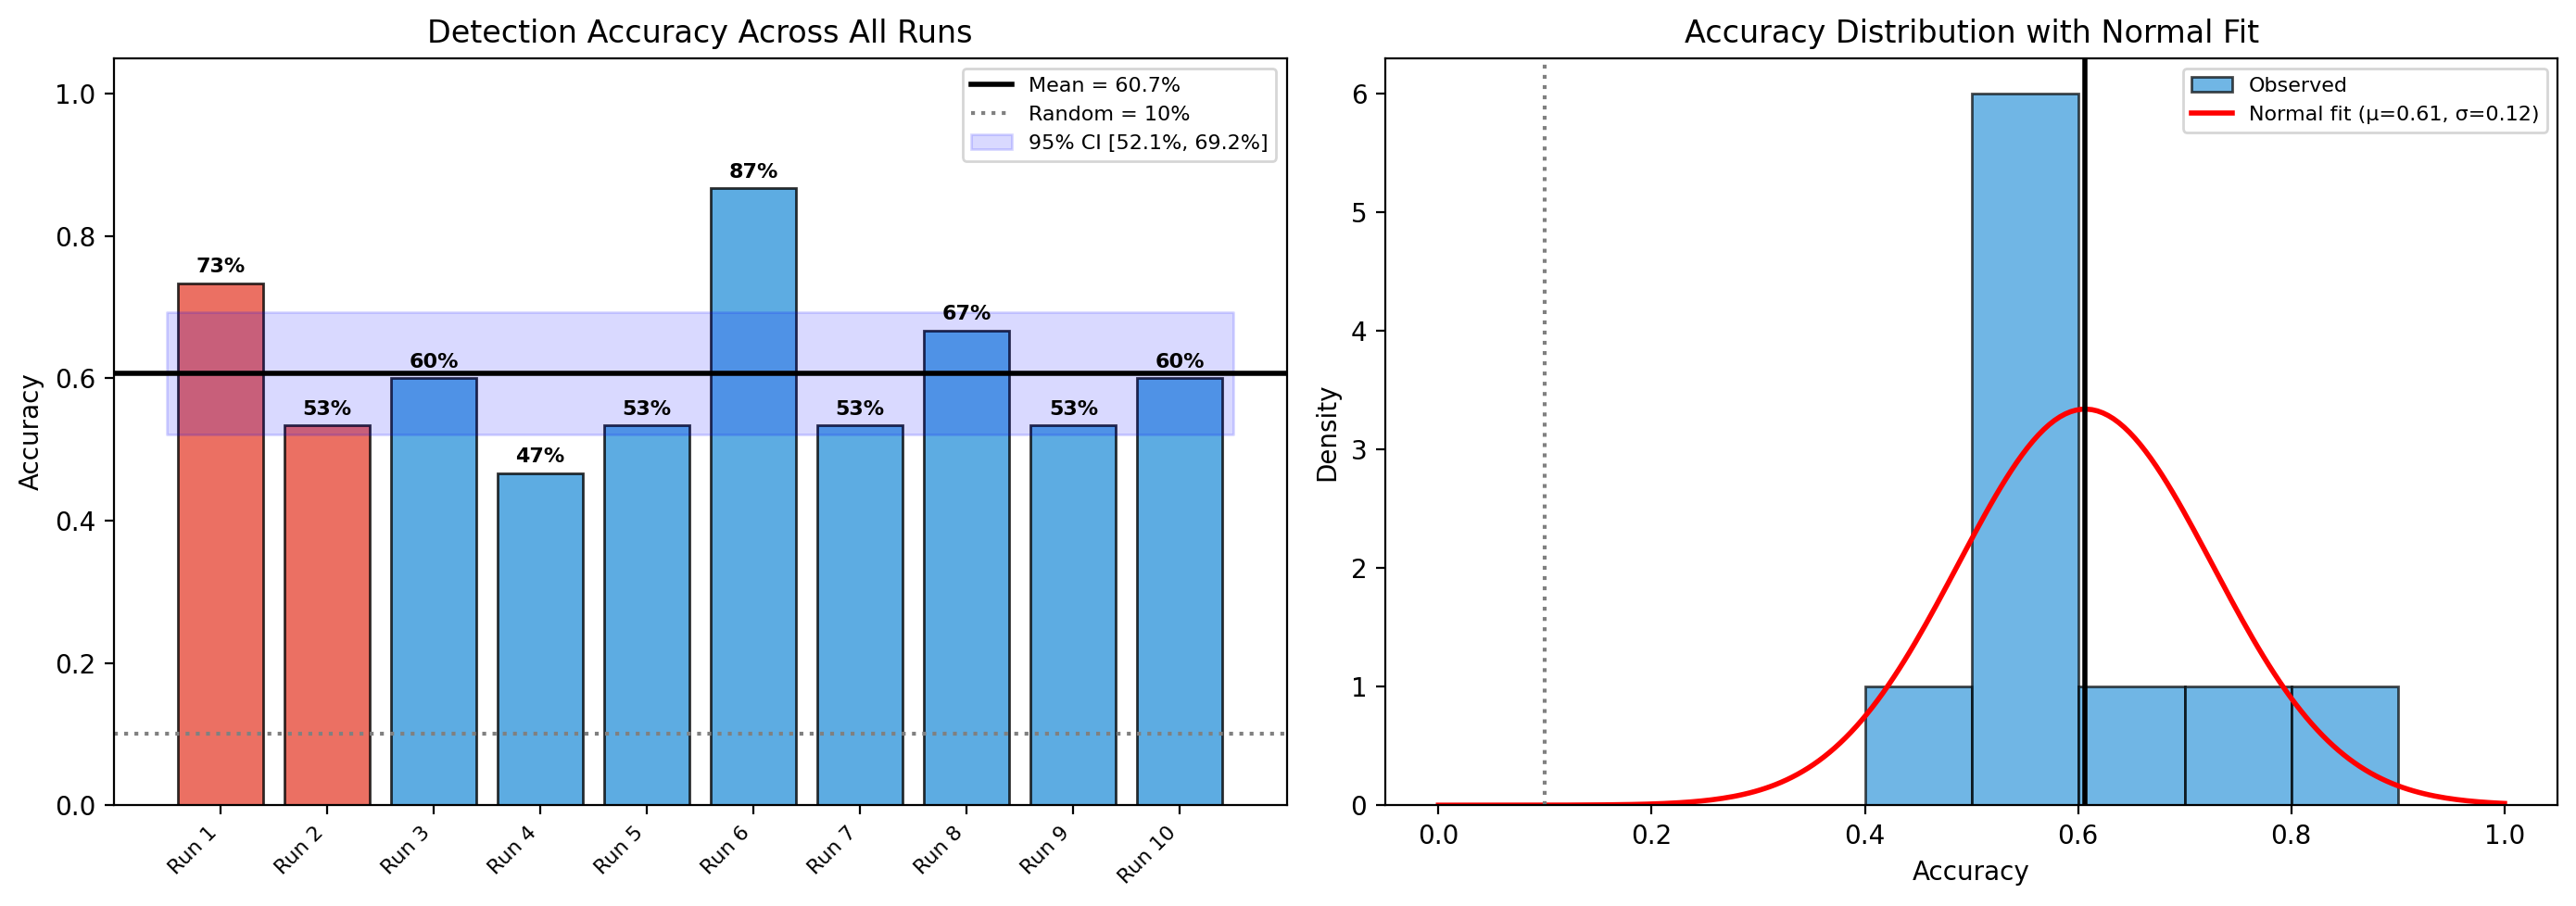
\includegraphics[width=\linewidth]{figures/fig1_accuracy_distribution.png}
    \Description{Bar chart of 10 run accuracies ranging from 47\% to 87\%, with a normal distribution fit showing mean 60.7\%.}
    \caption{Detection accuracy across all 10 runs. Left: per-run accuracy with mean and 95\% CI. Right: accuracy distribution with normal fit. The mean accuracy of 60.7\% is significantly above the 10\% random baseline ($t(9)=13.41$, $p < 0.001$).}
    \label{fig:accuracy_dist}
\end{figure}



\subsection{Per-Trial Learning Curve}

\begin{figure}[t]
    \centering
    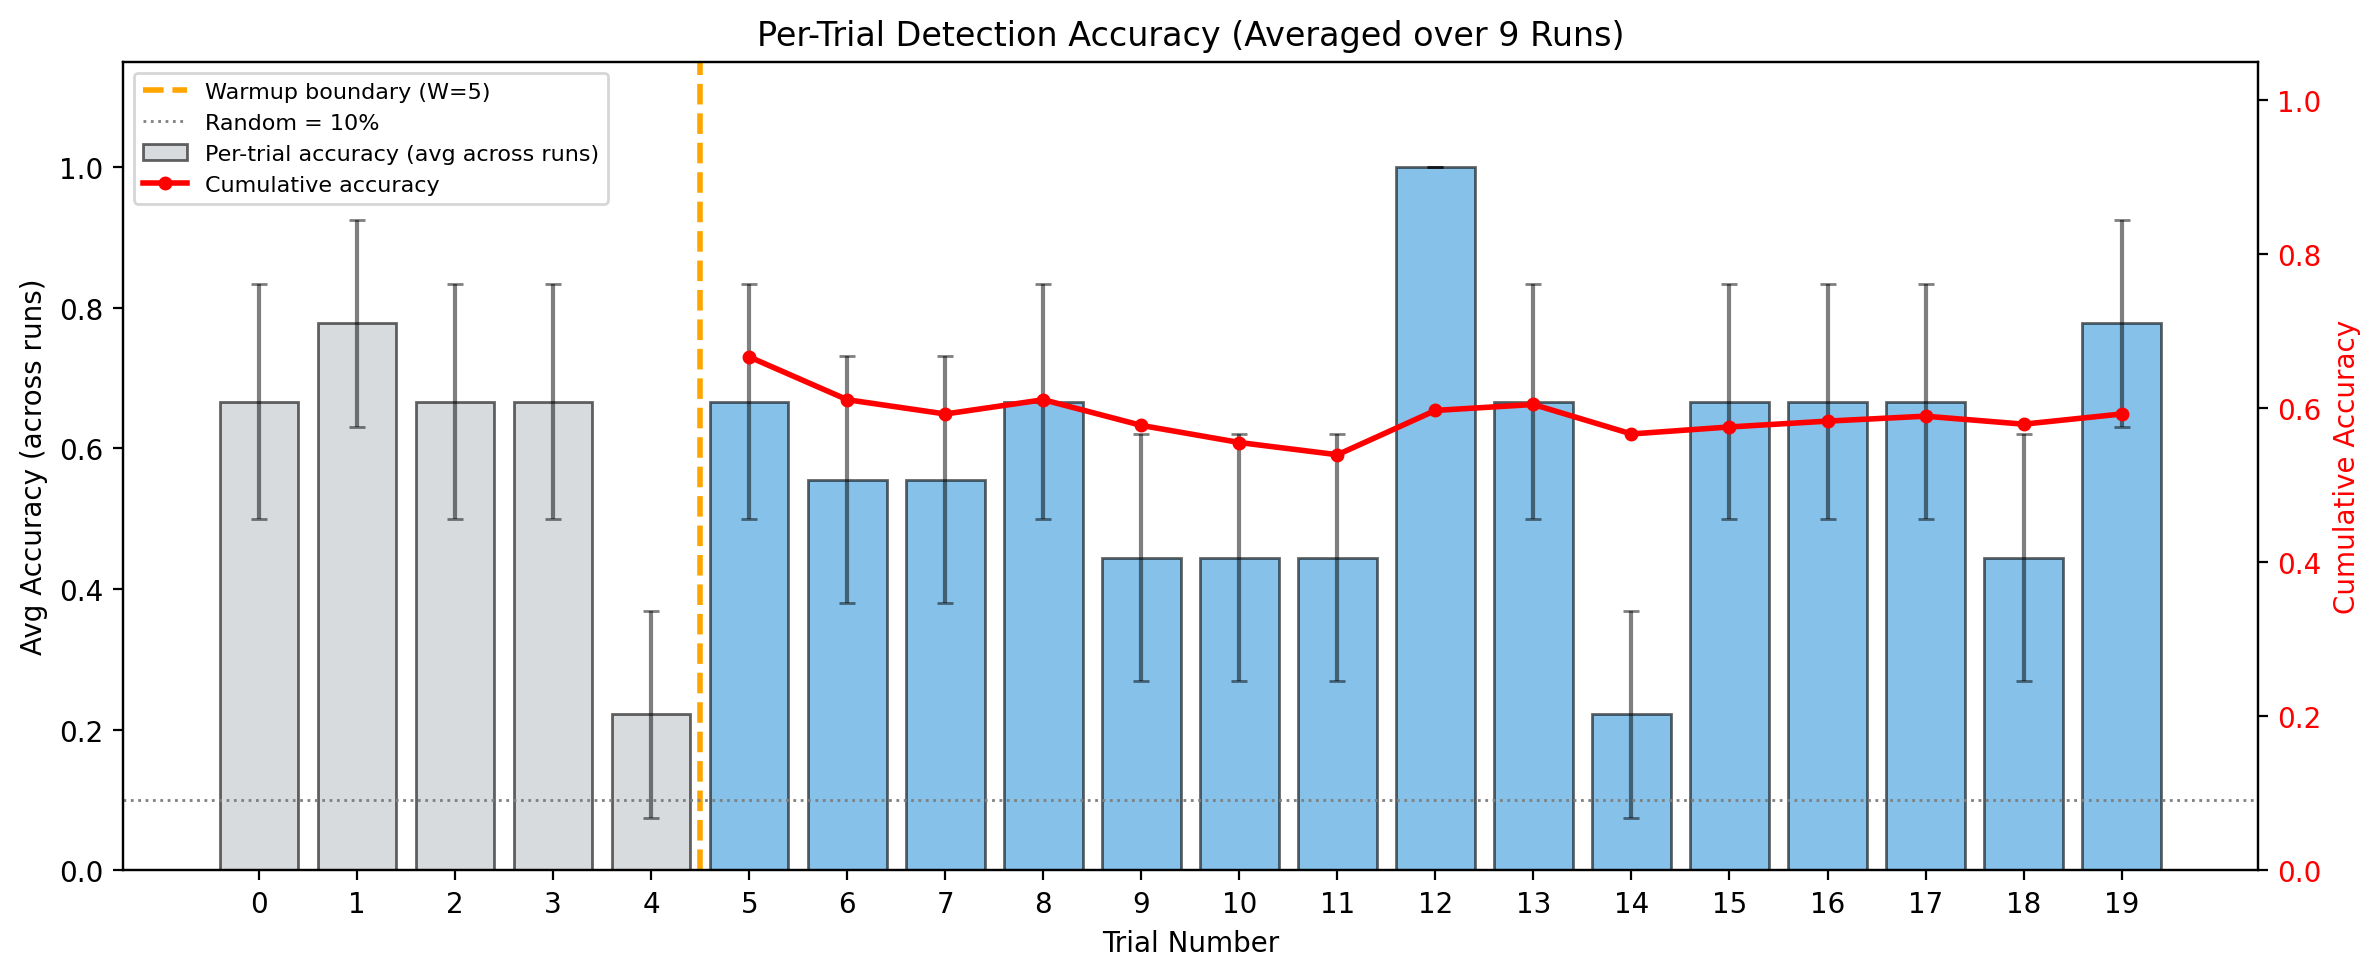
\includegraphics[width=\linewidth]{figures/fig2_per_trial_accuracy_curve.png}
    \Description{Bar chart with error bars showing per-trial accuracy across 20 trials, with a cumulative accuracy curve.}
    \caption{Per-trial detection accuracy averaged over 9 runs with full data. Blue bars show average accuracy at each trial position; the red curve shows cumulative accuracy from trial 5 onward. Error bars indicate standard error.}
    \label{fig:learning_curve}
\end{figure}

Figure~\ref{fig:learning_curve} shows the per-trial accuracy averaged across runs.
The first 5 trials serve as warmup.
The cumulative accuracy curve (red) shows the running average from trial 5 onward, revealing the Detective's performance trajectory as the Auditor iteratively refines its source text generation strategy.

\subsection{Per-Paraphraser Detection Rates}

\begin{figure}[t]
    \centering
    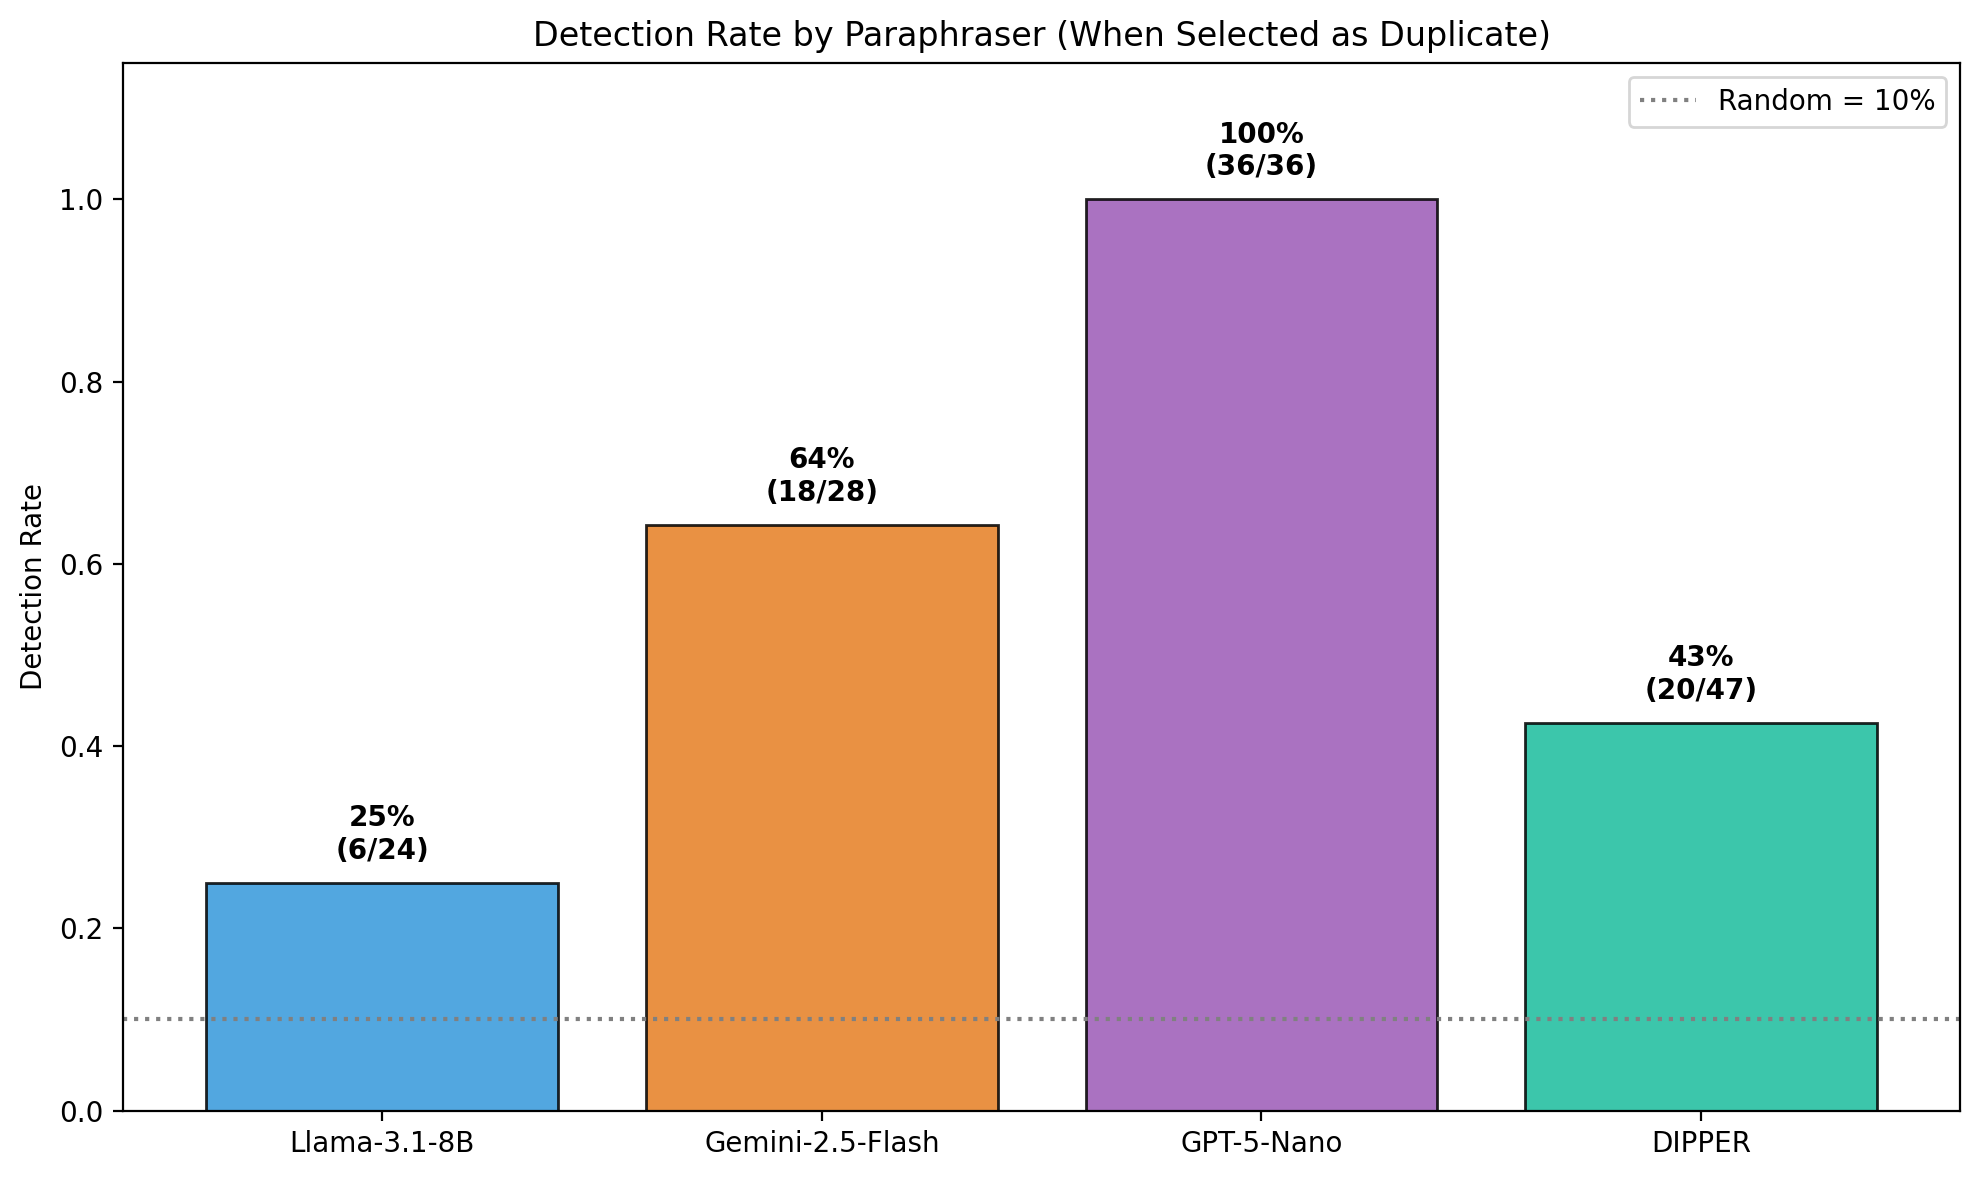
\includegraphics[width=\linewidth]{figures/fig3_paraphraser_detection_rate.png}
    \Description{Bar chart showing detection rates: Llama 25\%, Gemini 64\%, GPT-5-Nano 100\%, DIPPER 43\%.}
    \caption{Detection rate for each paraphraser when randomly selected as the duplicate source. GPT-5-Nano is detected with 100\% accuracy, while Llama-3.1-8B is hardest to detect at 25\%.}
    \label{fig:detection_rate}
\end{figure}

Detection rates vary dramatically across paraphrasers (Figure~\ref{fig:detection_rate}):

\begin{itemize}
    \item \textbf{GPT-5-Nano}: 100\% (36/36)---always detected when duplicated.
    \item \textbf{Gemini-2.5-Flash}: 64.3\% (18/28).
    \item \textbf{DIPPER}: 42.6\% (20/47).
    \item \textbf{Llama-3.1-8B}: 25.0\% (6/24)---hardest to detect.
\end{itemize}


\subsection{Confusion Analysis}

\begin{figure}[t]
    \centering
    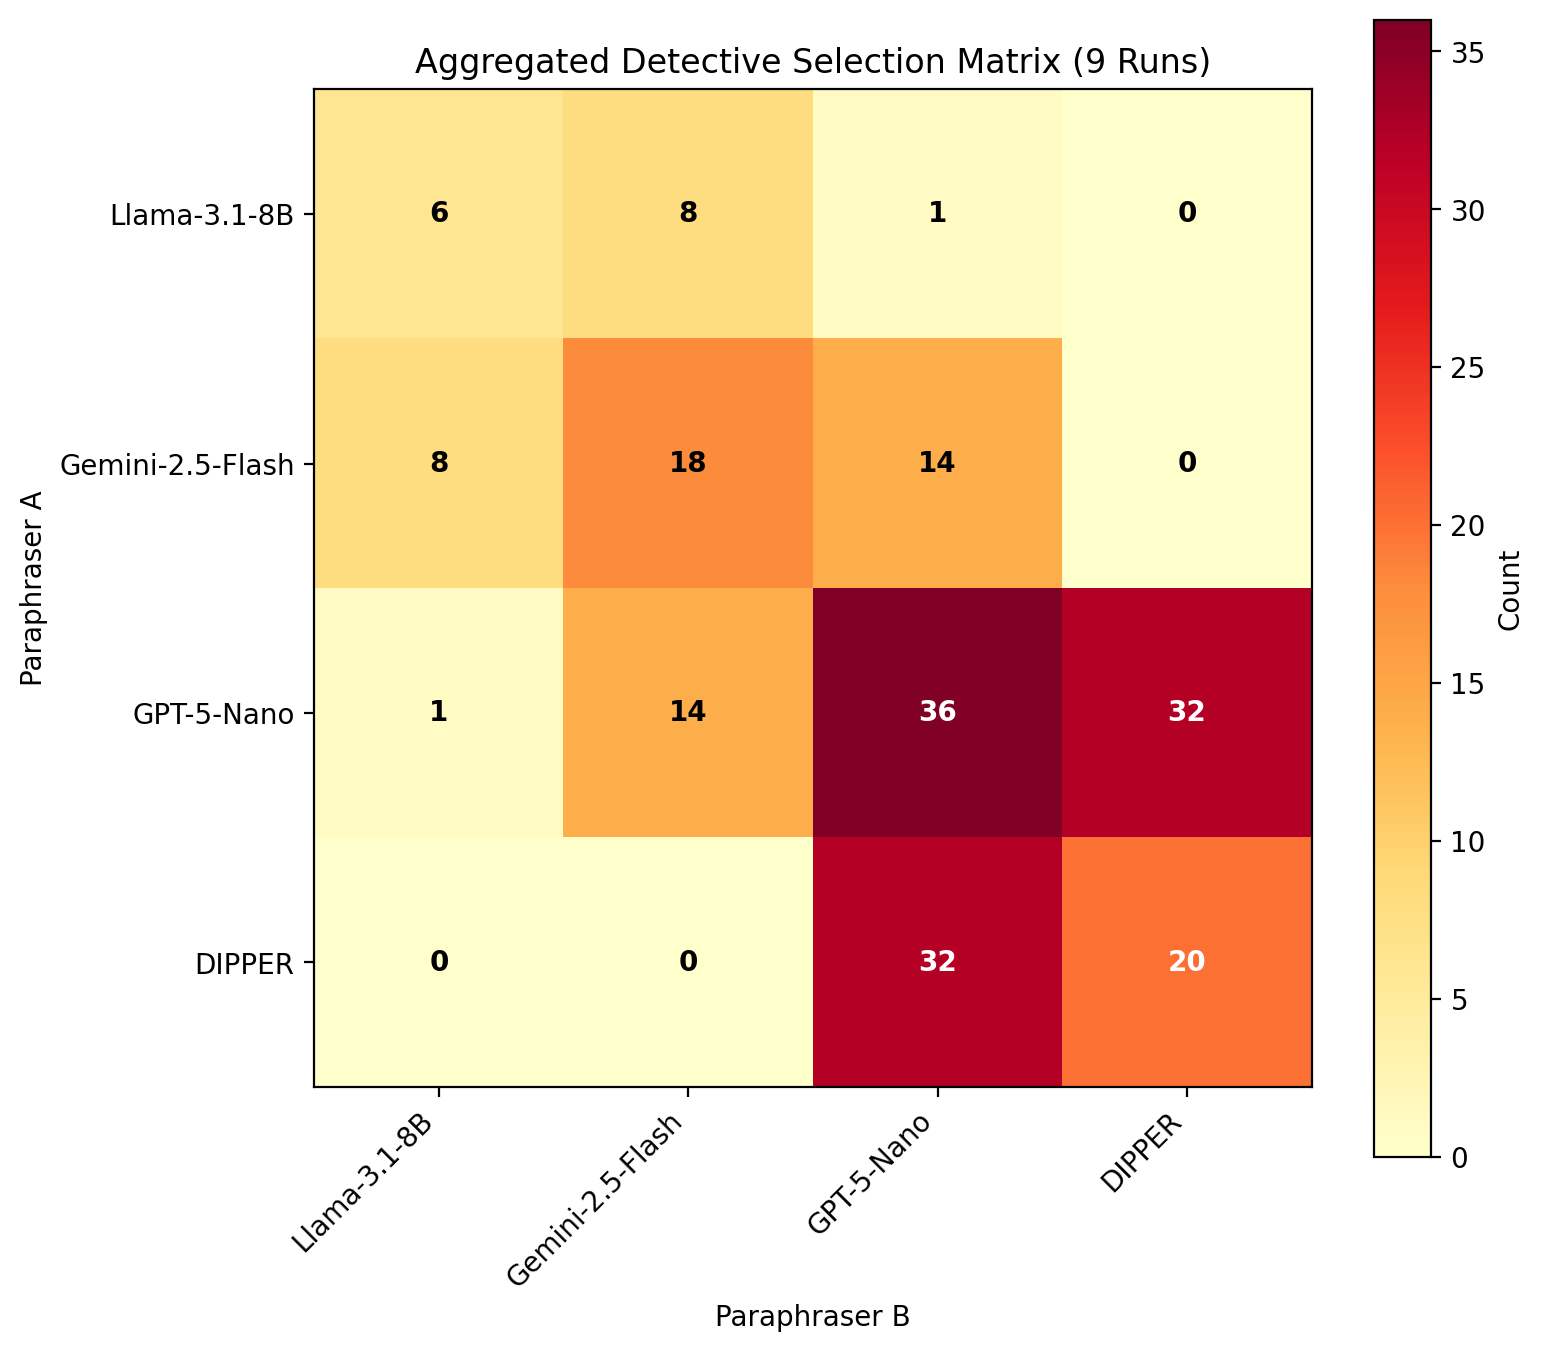
\includegraphics[width=0.85\linewidth]{figures/fig4_confusion_heatmap.png}
    \Description{4x4 heatmap showing paraphraser pair selection frequencies, with GPT-5-Nano diagonal at 36 and GPT-5-Nano--DIPPER off-diagonal at 32.}
    \caption{Aggregated confusion matrix showing how often the Detective paired each combination of paraphrasers. Diagonal entries represent correct identifications. The strong GPT-5-Nano--DIPPER off-diagonal (32) indicates the Detective frequently confuses these two.}
    \label{fig:confusion}
\end{figure}

The aggregated confusion matrix (Figure~\ref{fig:confusion}) reveals systematic patterns in the Detective's errors:

\begin{itemize}
    \item \textbf{GPT-5-Nano $\leftrightarrow$ DIPPER} (off-diagonal: 32): The most common confusion pair. Despite their architectural differences (LLM vs.\ T5-based), the Detective frequently groups their outputs together.
    \item \textbf{Gemini-2.5-Flash $\leftrightarrow$ GPT-5-Nano} (14): Moderate confusion between these two LLM-based paraphrasers.
    \item \textbf{Llama-3.1-8B $\leftrightarrow$ Gemini-2.5-Flash} (8): Some confusion between these models.
    \item \textbf{DIPPER $\leftrightarrow$ Llama-3.1-8B} (0): Never confused, suggesting maximally distinct fingerprints.
\end{itemize}

\subsection{Response Length as a Fingerprint Feature}

\begin{figure}[t]
    \centering
    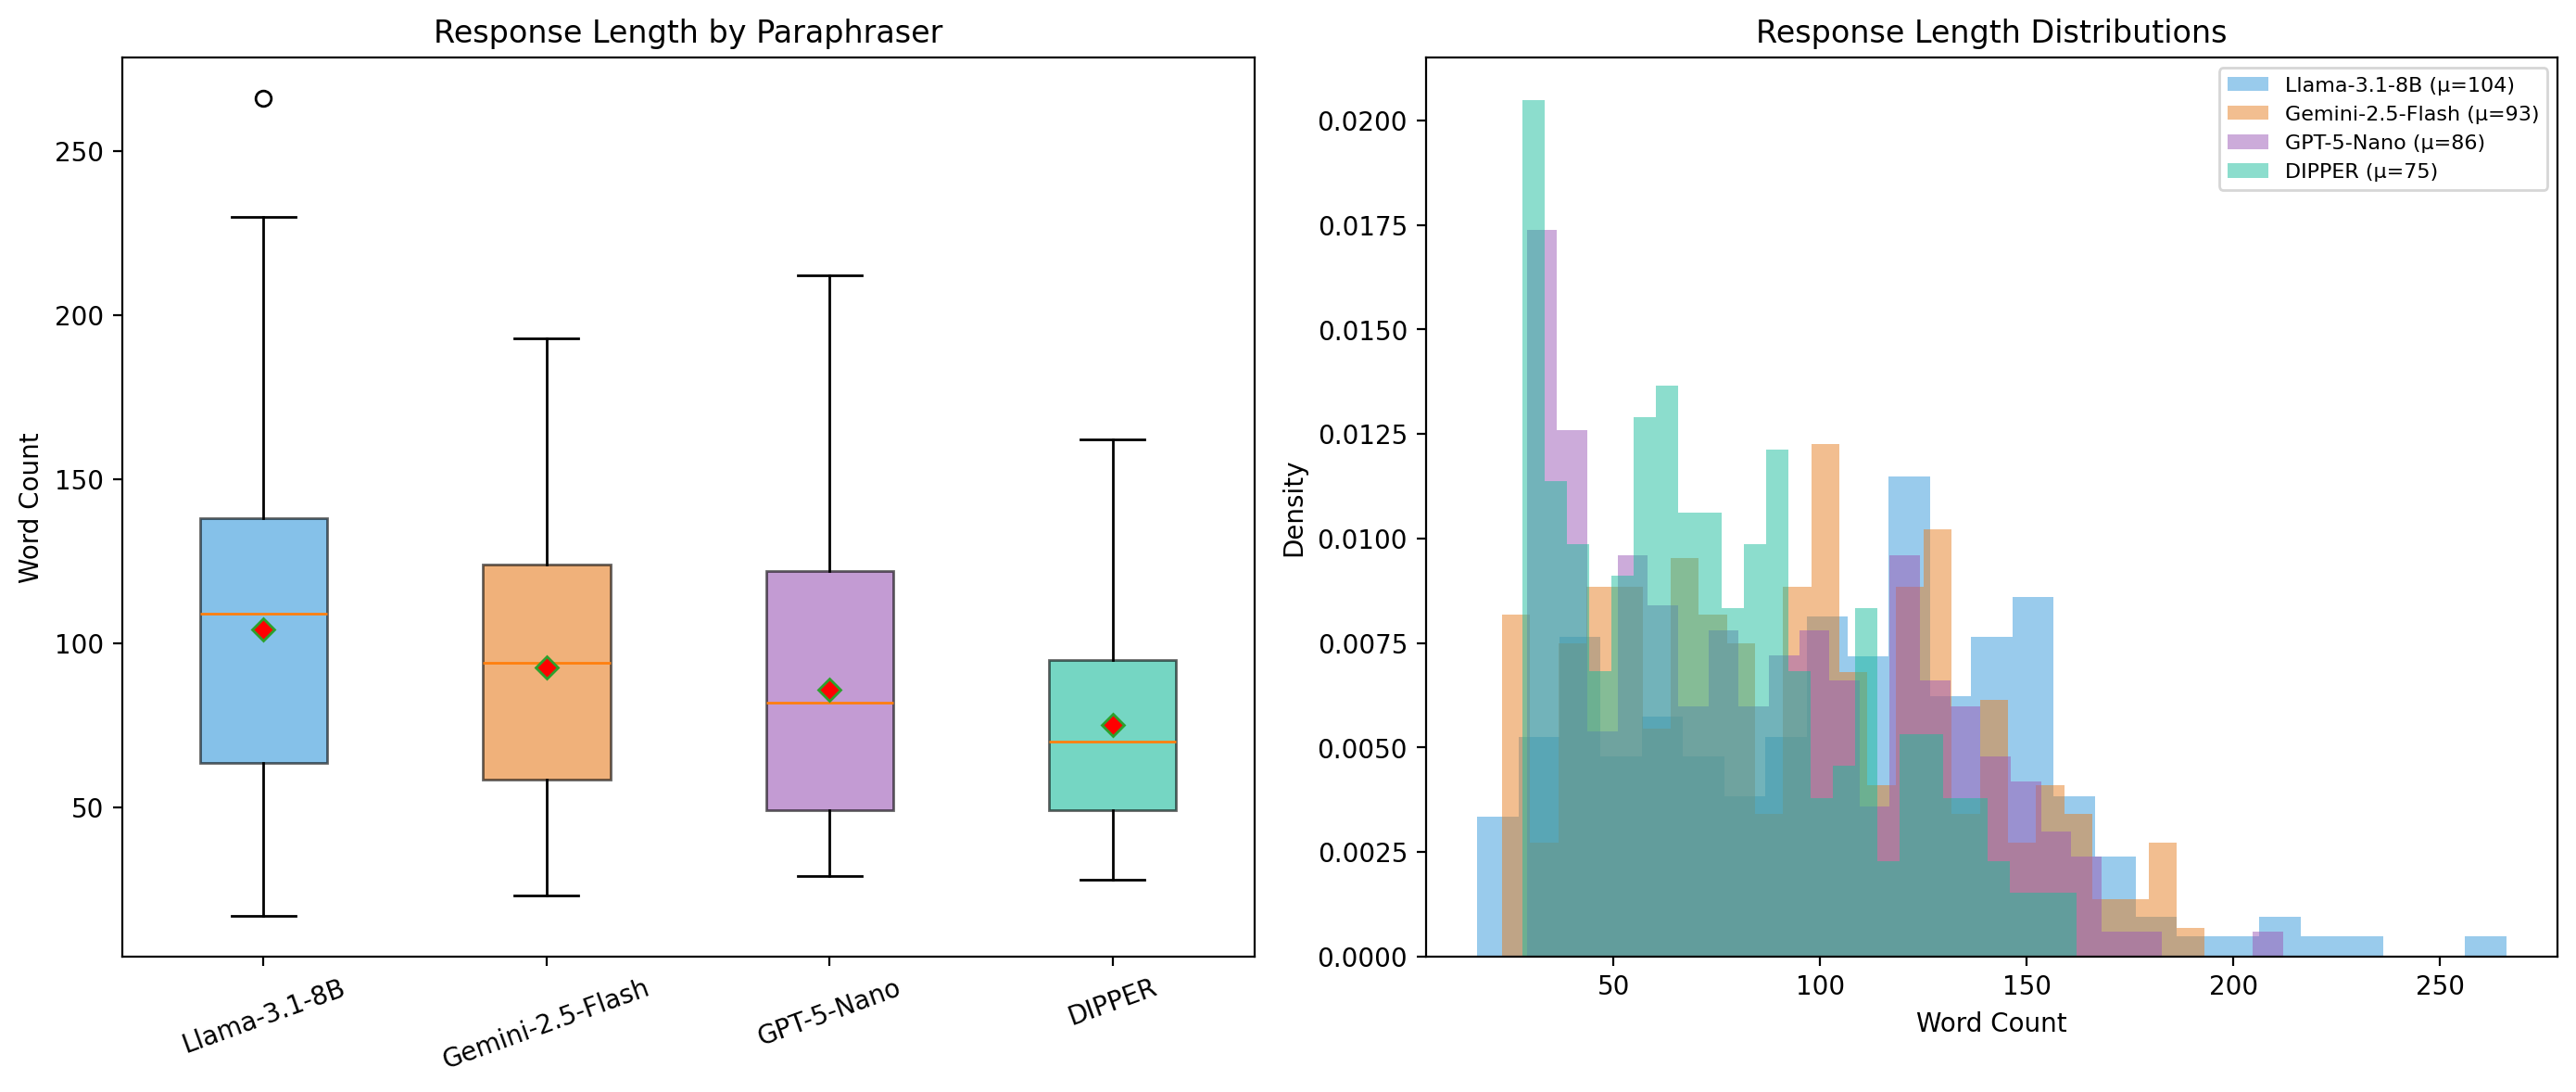
\includegraphics[width=\linewidth]{figures/fig5_response_length.png}
    \Description{Box plots and histograms of response word counts for four paraphrasers, ranging from mean 75 (DIPPER) to 104 (Llama).}
    \caption{Response length (word count) distributions per paraphraser. Left: box plots. Right: overlaid histograms. Llama-3.1-8B produces the longest outputs ($\mu=104$), while DIPPER produces the shortest ($\mu=75$).}
    \label{fig:response_length}
\end{figure}

Response length is a salient fingerprint dimension (Figure~\ref{fig:response_length}).
Table~\ref{tab:length_stats} summarizes the statistics.

\begin{table}[t]
\caption{Response length statistics (word count) per paraphraser.}
\label{tab:length_stats}
\centering
\begin{tabular}{lrrrr}
\toprule
\textbf{Paraphraser} & \textbf{Mean} & \textbf{Median} & \textbf{SD} & \textbf{$n$} \\
\midrule
Llama-3.1-8B     & 104 & 109 & 47 & 210 \\
Gemini-2.5-Flash & 93  & 94  & 41 & 216 \\
GPT-5-Nano       & 86  & 82  & 41 & 228 \\
DIPPER            & 75  & 70  & 33 & 246 \\
\bottomrule
\end{tabular}
\end{table}

DIPPER, as a T5-based model, produces the most conservative (shortest) paraphrases, while Llama-3.1-8B tends toward verbose, elaborative rewrites.
Interestingly, despite GPT-5-Nano having moderate length, its fingerprint is the strongest---suggesting that length alone is insufficient and that deeper stylistic features (word choice, sentence structure, formatting patterns) play a critical role.

\subsection{Source Text Type Comparison}

\begin{figure}[t]
    \centering
    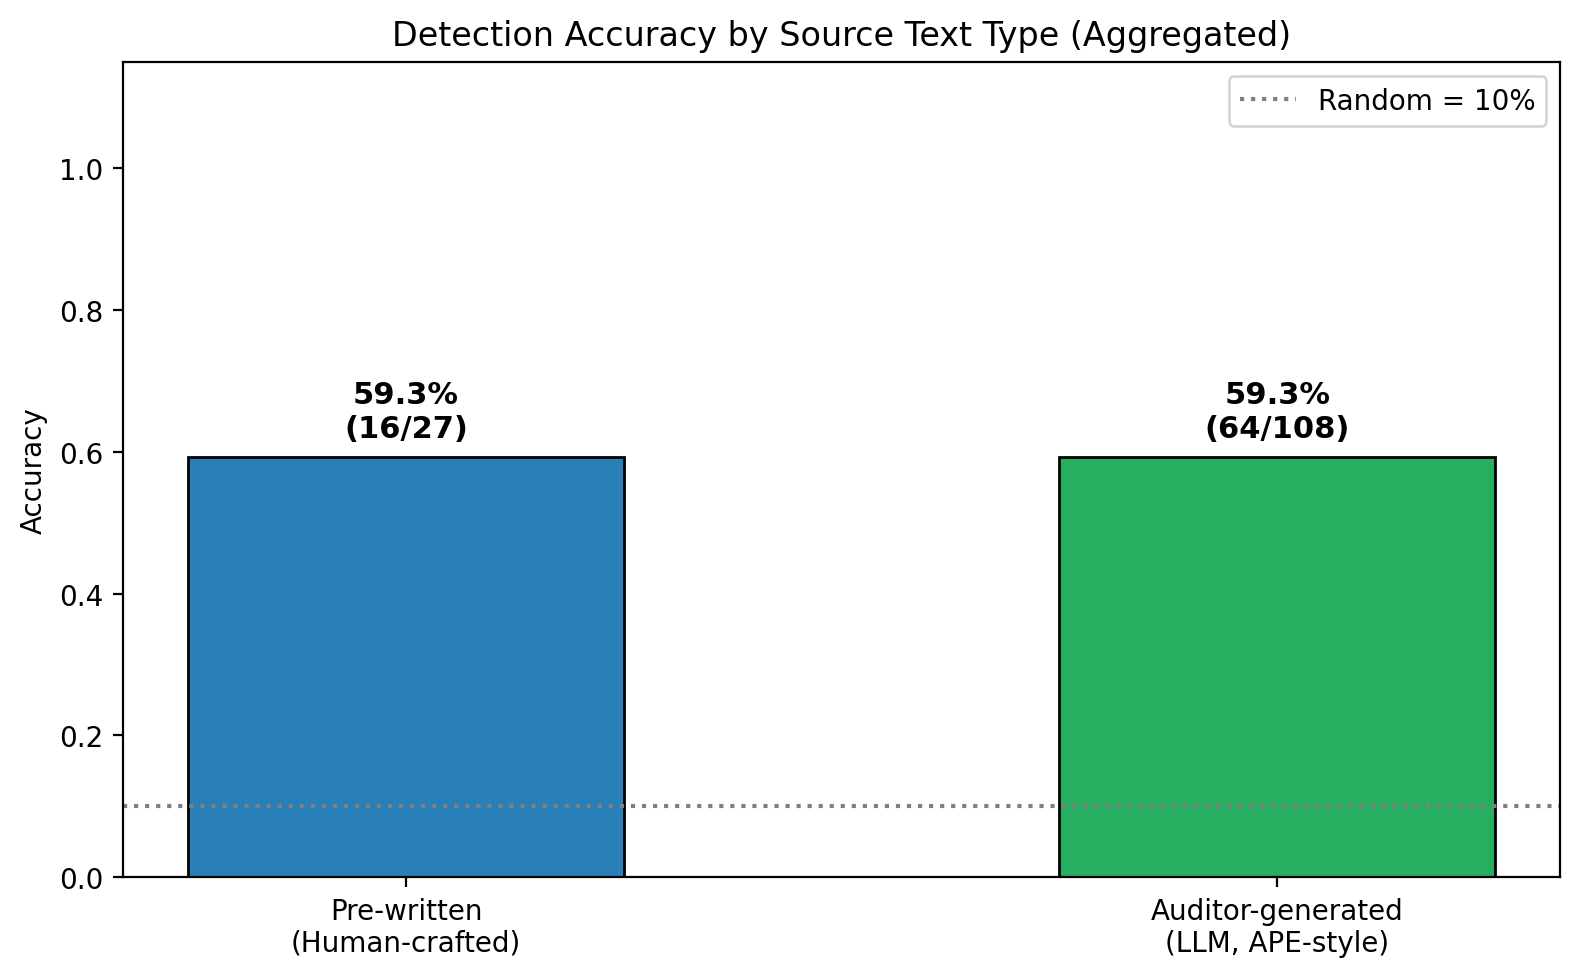
\includegraphics[width=0.85\linewidth]{figures/fig6_source_type_accuracy.png}
    \Description{Two-bar chart comparing pre-written (59.3\%) and auditor-generated (59.3\%) source text accuracy.}
    \caption{Detection accuracy by source text type. Both human-crafted and Auditor-generated texts yield identical accuracy (59.3\%), suggesting the APE-style refinement matches human-designed linguistic traps.}
    \label{fig:source_type}
\end{figure}



\subsection{Detective Rationale Analysis}

\begin{figure}[t]
    \centering
    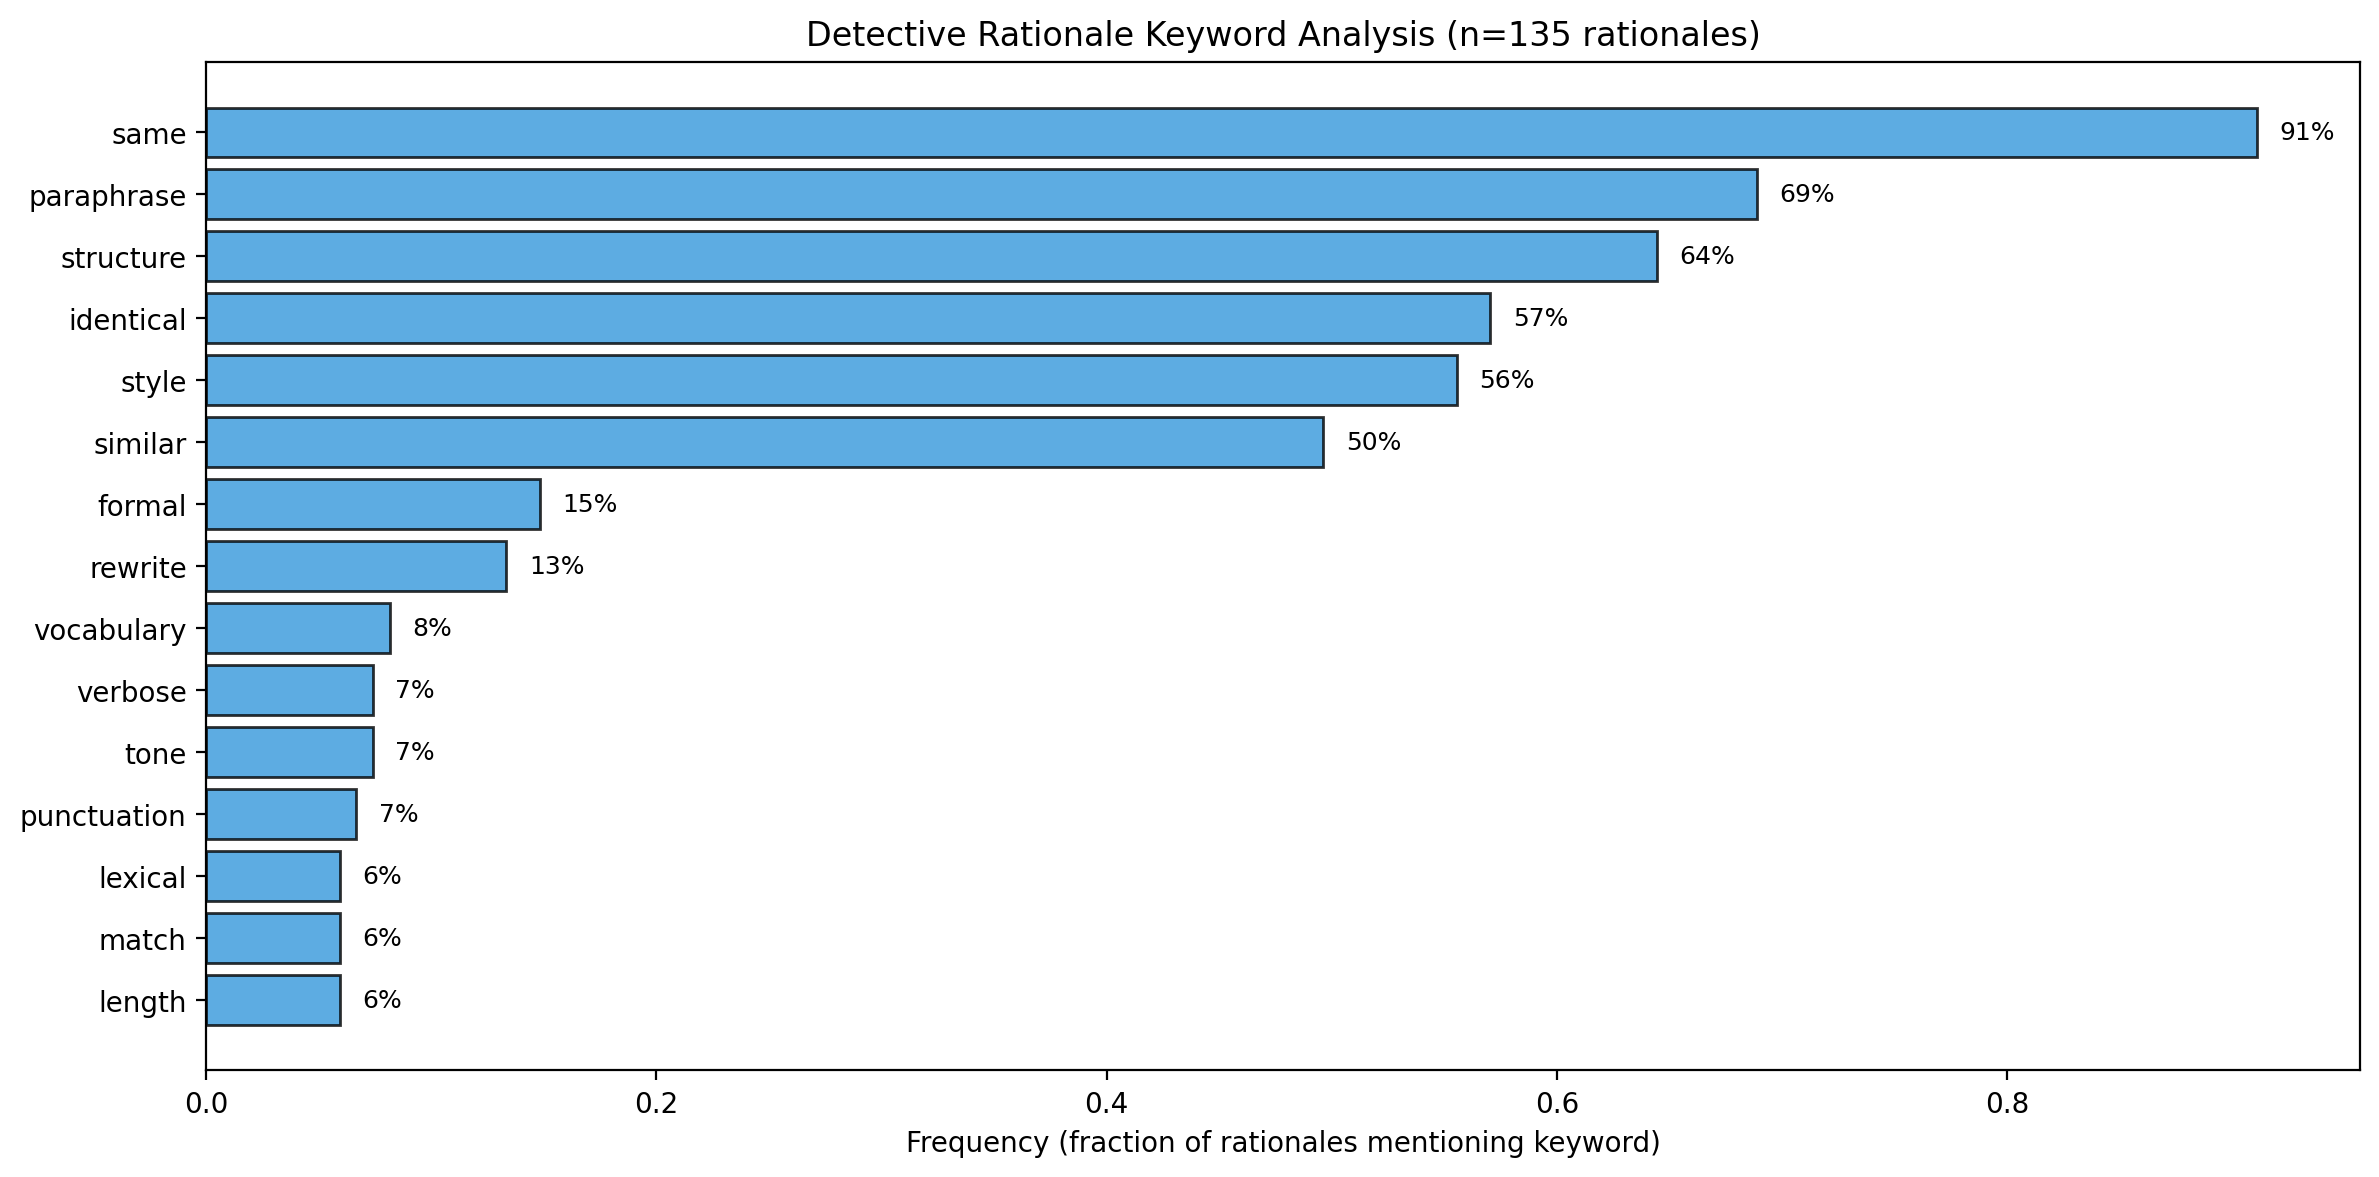
\includegraphics[width=\linewidth]{figures/fig8_rationale_keywords.png}
    \Description{Horizontal bar chart of keyword frequencies in detective rationales, with structure at 64\% and style at 56\%.}
    \caption{Keyword frequency analysis of Detective rationales ($n=135$). Structural and stylistic features dominate the Detective's reasoning.}
    \label{fig:rationale}
\end{figure}

Analysis of 135 Detective rationales reveals the features most relied upon for fingerprint identification (Figure~\ref{fig:rationale}):
\emph{structure} (64\%), \emph{style} (56\%), \emph{formal} (15\%), \emph{vocabulary} (8\%), \emph{tone} (7\%), and \emph{length} (6\%).
The dominance of structural and stylistic features over surface-level features like length confirms that the Detective performs genuine stylistic analysis rather than relying on trivial heuristics.


% ============================================================
\section{Plan for Next Steps}
% ============================================================

Based on our findings, we propose the following directions:

\begin{enumerate}
    \item \textbf{Upgrade Detective model.} Replace Paraphrasers or Auditor with a more capable model (e.g., Claude Opus, GPT-5) to test whether stronger reasoning improves fingerprint detection.
    \item \textbf{Expand paraphraser pool.} Add more paraphrasers (e.g., Mistral, Command-R, Qwen) to test whether fingerprinting scales to larger model sets and whether models from the same family (e.g., Llama-3.1-8B vs.\ Llama-3.1-70B) are distinguishable.
\end{enumerate}

% ============================================================
\section{Conclusion}
% ============================================================

\begin{itemize}
    \item Fingerprint strength varies dramatically across models: GPT-5-Nano is always detectable (100\%), while Llama-3.1-8B is rarely detected (25\%).
    \item The Detective relies primarily on structural and stylistic features rather than surface-level heuristics like output length.
\end{itemize}

These results suggest that the ``wood grain'' of AI models is real and measurable, opening avenues for paraphraser attribution, AI text provenance, and deeper understanding of how different architectures shape language generation.

\end{document}
